\documentclass[tikz,border=10pt]{standalone}
\usepackage{tikz}
\usetikzlibrary{positioning, arrows.meta, calc, patterns, decorations.pathreplacing}
\usepackage{amsmath}

\begin{document}
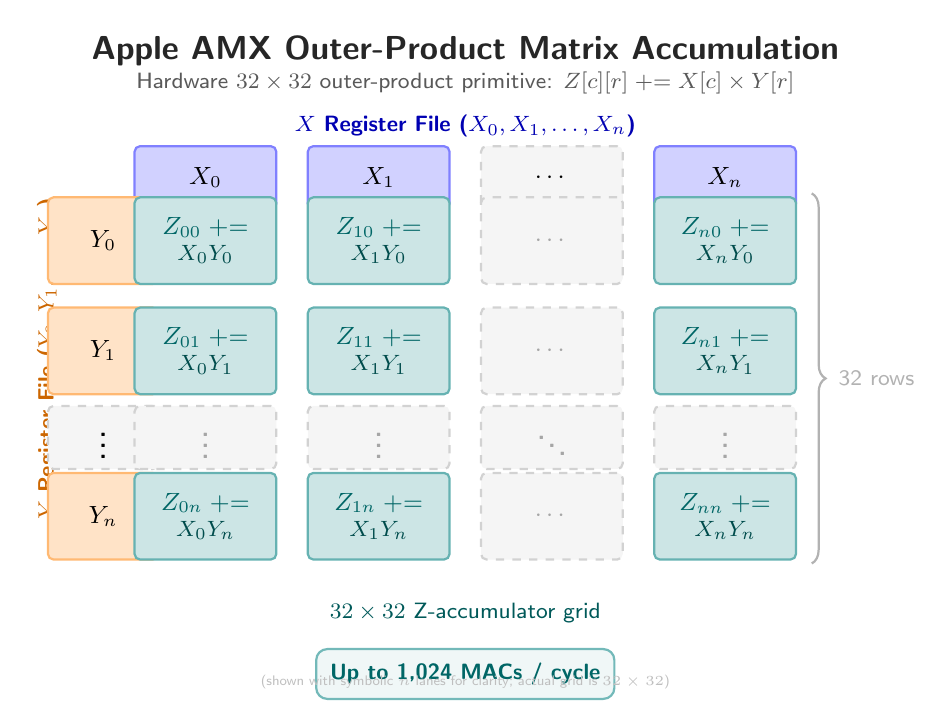
\begin{tikzpicture}[
    >=Stealth,
    font=\sffamily\small,
    cell active/.style={fill=teal!20, draw=teal!60, thick, rounded corners=2pt,
                        minimum width=18mm, minimum height=11mm, inner sep=2pt},
    cell dots/.style={fill=gray!8, draw=gray!35, dashed, thick, rounded corners=2pt,
                      minimum width=18mm, minimum height=11mm, inner sep=2pt},
    cell dots mid/.style={fill=gray!8, draw=gray!35, dashed, thick, rounded corners=2pt,
                          minimum width=18mm, minimum height=8mm, inner sep=2pt},
    reg x/.style={fill=blue!18, draw=blue!50, thick, rounded corners=2pt,
                  minimum width=18mm, minimum height=8mm, inner sep=2pt},
    reg x dots/.style={fill=gray!8, draw=gray!35, dashed, thick, rounded corners=2pt,
                       minimum width=18mm, minimum height=8mm, inner sep=2pt},
    reg y/.style={fill=orange!22, draw=orange!55, thick, rounded corners=2pt,
                  minimum width=14mm, minimum height=11mm, inner sep=2pt},
    reg y dots/.style={fill=gray!8, draw=gray!35, dashed, thick, rounded corners=2pt,
                       minimum width=14mm, minimum height=8mm, inner sep=2pt},
]

\def\gw{2.2}   % column pitch
\def\gh{1.4}   % row pitch
\def\mh{1.0}   % middle row pitch

% =====================================================================
% Title
% =====================================================================
\node[font=\sffamily\large\bfseries, text=black!85] at ({1.5*\gw}, 2.4)
    {Apple AMX Outer-Product Matrix Accumulation};
\node[font=\sffamily\footnotesize, text=gray!70!black] at ({1.5*\gw}, 2.0)
    {Hardware $32\times32$ outer-product primitive: $Z[c][r] \mathrel{+}= X[c] \times Y[r]$};

% =====================================================================
% Top: X register vector
% =====================================================================
\node[font=\sffamily\footnotesize\bfseries, text=blue!70!black] at ({1.5*\gw}, 1.45)
    {$X$ Register File ($X_0, X_1, \dots, X_n$)};

\node[reg x] (X0) at (0, 0.8) {\bfseries $X_0$};
\node[reg x] (X1) at (\gw, 0.8) {\bfseries $X_1$};
\node[reg x dots] (Xm) at ({2*\gw}, 0.8) {\bfseries $\cdots$};
\node[reg x] (Xn) at ({3*\gw}, 0.8) {\bfseries $X_n$};

% Downward flow arrows
\draw[blue!45, thick, ->] (X0.south) -- ++(0, -0.35);
\draw[blue!45, thick, ->] (X1.south) -- ++(0, -0.35);
\draw[blue!45, thick, ->] (Xn.south) -- ++(0, -0.35);

% =====================================================================
% Left: Y register vector
% =====================================================================
\node[rotate=90, font=\sffamily\footnotesize\bfseries, text=orange!80!black] at (-2.0, -1.5)
    {$Y$ Register File ($Y_0, Y_1, \dots, Y_n$)};

\node[reg y] (Y0) at (-1.3, 0) {\bfseries $Y_0$};
\node[reg y] (Y1) at (-1.3, -\gh) {\bfseries $Y_1$};
\node[reg y dots] (Ym) at (-1.3, {-2*\gh + 0.3}) {\bfseries $\vdots$};
\node[reg y] (Yn) at (-1.3, {-2*\gh - \mh + 0.3}) {\bfseries $Y_n$};

% Rightward flow arrows
\draw[orange!50, thick, ->] (Y0.east) -- ++(0.35, 0);
\draw[orange!50, thick, ->] (Y1.east) -- ++(0.35, 0);
\draw[orange!50, thick, ->] (Yn.east) -- ++(0.35, 0);

% =====================================================================
% Center: Z Accumulator Matrix
% =====================================================================
% Row 0 (Y0)
\node[cell active] at (0, 0) {\shortstack[c]{\bfseries\color{teal!80!black} $Z_{00} \mathrel{+}=$\\\footnotesize\color{teal!60!black} $X_0 Y_0$}};
\node[cell active] at (\gw, 0) {\shortstack[c]{\bfseries\color{teal!80!black} $Z_{10} \mathrel{+}=$\\\footnotesize\color{teal!60!black} $X_1 Y_0$}};
\node[cell dots] at ({2*\gw}, 0) {\bfseries\color{gray!70} $\cdots$};
\node[cell active] at ({3*\gw}, 0) {\shortstack[c]{\bfseries\color{teal!80!black} $Z_{n0} \mathrel{+}=$\\\footnotesize\color{teal!60!black} $X_n Y_0$}};

% Row 1 (Y1)
\node[cell active] at (0, -\gh) {\shortstack[c]{\bfseries\color{teal!80!black} $Z_{01} \mathrel{+}=$\\\footnotesize\color{teal!60!black} $X_0 Y_1$}};
\node[cell active] at (\gw, -\gh) {\shortstack[c]{\bfseries\color{teal!80!black} $Z_{11} \mathrel{+}=$\\\footnotesize\color{teal!60!black} $X_1 Y_1$}};
\node[cell dots] at ({2*\gw}, -\gh) {\bfseries\color{gray!70} $\cdots$};
\node[cell active] at ({3*\gw}, -\gh) {\shortstack[c]{\bfseries\color{teal!80!black} $Z_{n1} \mathrel{+}=$\\\footnotesize\color{teal!60!black} $X_n Y_1$}};

% Row 2 (Middle dots)
\node[cell dots mid] at (0, {-2*\gh + 0.3}) {\bfseries\color{gray!70} $\vdots$};
\node[cell dots mid] at (\gw, {-2*\gh + 0.3}) {\bfseries\color{gray!70} $\vdots$};
\node[cell dots mid] at ({2*\gw}, {-2*\gh + 0.3}) {\bfseries\color{gray!70} $\ddots$};
\node[cell dots mid] at ({3*\gw}, {-2*\gh + 0.3}) {\bfseries\color{gray!70} $\vdots$};

% Row 3 (Yn)
\node[cell active] at (0, {-2*\gh - \mh + 0.3}) {\shortstack[c]{\bfseries\color{teal!80!black} $Z_{0n} \mathrel{+}=$\\\footnotesize\color{teal!60!black} $X_0 Y_n$}};
\node[cell active] at (\gw, {-2*\gh - \mh + 0.3}) {\shortstack[c]{\bfseries\color{teal!80!black} $Z_{1n} \mathrel{+}=$\\\footnotesize\color{teal!60!black} $X_1 Y_n$}};
\node[cell dots] at ({2*\gw}, {-2*\gh - \mh + 0.3}) {\bfseries\color{gray!70} $\cdots$};
\node[cell active] at ({3*\gw}, {-2*\gh - \mh + 0.3}) {\shortstack[c]{\bfseries\color{teal!80!black} $Z_{nn} \mathrel{+}=$\\\footnotesize\color{teal!60!black} $X_n Y_n$}};

% Brace on the right
\draw[decorate, decoration={brace, amplitude=5pt, mirror}, thick, gray!60]
    ({3*\gw + 1.1}, {-2*\gh - \mh - 0.3})
    -- node[right=6pt, font=\sffamily\footnotesize, text=gray!60] {32 rows}
    ({3*\gw + 1.1}, 0.6);

% =====================================================================
% Bottom Labels and Badge
% =====================================================================
\node[below=8pt, font=\sffamily\footnotesize, text=teal!70!black]
    at ({1.5*\gw}, {-2*\gh - \mh - 0.4})
    {$32\times32$ Z-accumulator grid};

\node[below=22pt, draw=teal!55, fill=teal!6, thick, rounded corners=4pt,
      font=\sffamily\footnotesize\bfseries, inner sep=5pt, text=teal!80!black]
    at ({1.5*\gw}, {-2*\gh - \mh - 0.6})
    {Up to 1,024 MACs / cycle};

\node[font=\sffamily\tiny, text=gray!50]
    at ({1.5*\gw}, {-2*\gh - \mh - 1.8})
    {(shown with symbolic $n$ lanes for clarity; actual grid is $32\times32$)};

\end{tikzpicture}
\end{document}
